
\documentclass[twoside]{article}
\setlength{\oddsidemargin}{0.25 in}
\setlength{\evensidemargin}{-0.25 in}
\setlength{\topmargin}{-0.6 in}
\setlength{\textwidth}{6.5 in}
\setlength{\textheight}{8.5 in}
\setlength{\headsep}{0.75 in}
\setlength{\parindent}{0 in}
\setlength{\parskip}{0.1 in}
\setlength{\parindent}{0pt}
\newcommand{\forceindent}{\leavevmode{\parindent=1em\indent}}
\usepackage{hyperref}
\usepackage{amsmath,amsfonts,graphicx}
\usepackage{subfig}

\newcounter{lecnum}
\renewcommand{\thepage}{\thelecnum-\arabic{page}}
\renewcommand{\thesection}{\thelecnum.\arabic{section}}
\renewcommand{\theequation}{\thelecnum.\arabic{equation}}
\renewcommand{\thefigure}{\thelecnum.\arabic{figure}}
\renewcommand{\thetable}{\thelecnum.\arabic{table}}

\newcommand{\lecture}[4]{
   \pagestyle{myheadings}
   \thispagestyle{plain}
   \newpage
   \setcounter{lecnum}{#1}
   \setcounter{page}{1}
   \noindent
   \begin{center}
   \framebox{
      \vbox{\vspace{2mm}
    \hbox to 6.28in { {\bf Information Retrieval and Web Agents: Final Project
	\hfill Spring 2017} }
       \vspace{4mm}
       \hbox to 6.28in { {\Large \hfill Course Search Engine for Semester.ly  \hfill} }
       \vspace{2mm}
       \hbox to 6.28in { {\it Lecturer: #3 \hfill Student: #4} }
      \vspace{2mm}}
   }
   \end{center}
   \markboth{}{}
}

\renewcommand{\cite}[1]{[#1]}
\def\beginrefs{\begin{list}%
        {[\arabic{equation}]}{\usecounter{equation}
         \setlength{\leftmargin}{2.0truecm}\setlength{\labelsep}{0.4truecm}%
         \setlength{\labelwidth}{1.6truecm}}}
\def\endrefs{\end{list}}
\def\bibentry#1{\item[\hbox{[#1]}]}

%Use this command for a figure; it puts a figure in wherever you want it.
%usage: \fig{NUMBER}{SPACE-IN-INCHES}{CAPTION}
\newcommand{\fig}[3]{
			\vspace{#2}
			\begin{center}
			Figure \thelecnum.#1:~#3=
			\end{center}
	}
% Use these for theorems, lemmas, proofs, etc.
\newtheorem{theorem}{Theorem}[lecnum]
\newtheorem{lemma}[theorem]{Lemma}
\newtheorem{proposition}[theorem]{Proposition}
\newtheorem{claim}[theorem]{Claim}
\newtheorem{corollary}[theorem]{Corollary}
\newtheorem{definition}[theorem]{Definition}
\newenvironment{proof}{{\bf Proof:}}{\hfill\rule{2mm}{2mm}}

\newcommand\E{\mathbb{E}}

\begin{document}
\lecture{1}{March 20}{Dr. David Yarowsky}{SangHyeon (Alex) Ahn}

\section{Abstract}

Semester.ly is a web application developed by students of Johns Hopkins University that enables college students to efficiently manage their timetables for courses. Semester.ly currently supports 9 different colleges with thousands of active users with more than a billion searches per year. At this moment, the web's course search is made based on the keywords matches between user's query and titles of courses, which is a simple boolean index search method. In this project, we intend to expand the scope of search beyond course titles, retrieving most relevant courses to users' queries based on advanced information retrieval techniques. In this project, course corpus is transformed to document vectors using variety of methods including N-gram sequence of words, term weightings, stopwords, word embedding and more. In our case study, we use precision/recall scores to evaluate each retrieval method's effectiveness.

\section{Objective}

Objective of the project is simple: to provide a functionality that serves users to retrieve the most relevant courses based on a query typed in a search bar on Semester.ly. I would like to expand the range of user-typed-query to fetch beyond the course titles, including course description, evaluations, instructors, level of difficulty, and flexibility using appropriate information retrieval methods.

Current system of Semester.ly has a search engine that enlists courses that match with words typed in the search bar. Currently, search bar only returns the courses that fully contains query's tokens in their titles. Indeed, this limits users to explore and find courses that are beyond what it says by the title. For example, if a user types in "web robots", current system retrieves no courses, however, we can achieve to return "Information Retreival and Web Agents" class using our implementation.I believe that if we can extend the range of query from course titles to more broad and specific queries, the user experience will excel through more dynamic and useful course searches.

Going further, we shall explore the following objectives for enhancing the model.

\begin{enumerate}
\item Document Modeling
\item Document Modeling Expansion
\item Model evaluation using multiple metrics
\item Efficiency Optimization
\item Web Interface Implementation
\item Topic Modeling (Latent Dirichilet Allocation) 
\item Course clustering using topic feature transformation
\end{enumerate}

\section{Methodology: Document Retrieval}

In order to implement the Courses Search Engine, we make use of effective document retrieval method based on document-vector modeling.

Document-vector modeling is a way to encode each document (collective pieces of information for each course) from courses corpus (pertaining to each school) to perform tasks such as relevance ranking, clustering, and possibly classification. Our primary goal is relevance ranking. 

Relevance ranking is a way to sort relevant documents from a query, with respect to similarity scores. By computing similarity scores in various ways (i.e. cosine similarity, jaccard similarity, overlap similarity, dice similarity), one can retrieve most relevant courses based on user input query (or another course).

By default, we start with common bag-of-words document modeling for retrieval, then we add multiple features to refine/advance our search results in the following fields:

\begin{enumerate}
\item \textbf{Stopwords}\\
: using stopwords to eliminate non-meaningful words during search
\item \textbf{Stemming}\\
: stemming both queries and course document vectors (Porter Stemming) for improving vector modeling
\item \textbf{N-grams}\\
: utilizing different N-grams sequence of words for more accurate/specific query-searching (improving upon bag-of-words assumption).
\item \textbf{Term Frequency Weighting}\\
: accounting for Term Frequency - Inverse Document Frequency to normalize word distribution under corpus
\item \textbf{Term Area Weighting} \\
: weighting terms under different areas differently (i.e. giving more weights for tokens from course titles, than descriptions/evalutaions)
\end{enumerate}


For example, a query search may look as below (examplified using terminal).

\begin{verbatim}

Query: "object oriented software"

Results (Course : Similarity Score):

- Object Oriented Software Engineering: 1.48799391725
- Software Systems Engineering: 0.53881590608
- Software Engineering Management: 0.428571428571
- Software Vulnerability Analysis: 0.350523742702
- Examining Archaeological Objects: 0.315244162496
- Human Sexual Orientation: 0.297219149139
- Introductory Programming in Java: 0.274075483931
- Music Notation Software: 0.258198889747
- Pseudorandomness and Combinatorial Constructions: 0.182913228255
- Rehabilitation Engineering Seminar: 0.139009609371

\end{verbatim}

\section{Evaluations of Model}

For evaludation of our model, we use pre-defined queries and relevant courses to calculate precision/recall scores for each model.

Pre-defined sets of query and relevant courses resembles the following:

\begin{verbatim}
Query: python jupyter notebook data visualization-

Relevant Courses: EN.553.436, AS.171.205, AS.191.383, EN.625.740, EN.553.636
\end{verbatim}

Similar to how we made evaluations on each model, we calculate the following fields as measures of effectiveness.

\begin{enumerate}
\item Precision Scores at 0.25
\item Precision Scores at 0.50
\item Precision Scores at 0.70
\item Precision Scores at 1.00
\item Precision Mean1
\item Predicion Mean 2
\item Normalized Precision
\item Normalized Recall
\end{enumerate}

Scores are computed for each query and result, then average results are calculated to evaluate a model for each implementation change.

\vfill

\textbf{Basic Sequential Search (database course order)}
\begin{verbatim}
   ----------------------------------------------------------------
                          Averaged Results
   ----------------------------------------------------------------
   **  P.25   P.50   P.75   P1.00   P_mean1   P_mean2.  P_norm  R_norm
   ==  ====   ====   ====   =====   =======   ========  ======  ======
   14  0.00   0.00   0.00   0.00    0.0000    0.0000    0.197   0.515
\end{verbatim}

\textbf{Baseline Model (keyword boolean search)}
\begin{verbatim}
   ----------------------------------------------------------------
                          Averaged Results
   ----------------------------------------------------------------
   **  P.25   P.50   P.75   P1.00   P_mean1   P_mean2.  P_norm  R_norm
   ==  ====   ====   ====   =====   =======   ========  ======  ======
   14  0.14   0.14   0.14   0.15    0.1429    0.1429    0.195   0.514
\end{verbatim}

\textbf{Basic Document Vector Model (raw term frequency)}
\begin{verbatim}
   ----------------------------------------------------------------
                          Averaged Results
   ----------------------------------------------------------------
   **  P.25   P.50   P.75   P1.00   P_mean1   P_mean2.  P_norm  R_norm
   ==  ====   ====   ====   =====   =======   ========  ======  ======
   14  0.32   0.25   0.26   0.22    0.2778    0.2783    0.653   0.846
\end{verbatim}


\textbf{Basic + Stemming}
\begin{verbatim}
   ----------------------------------------------------------------
                          Averaged Results
   ----------------------------------------------------------------
   **  P.25   P.50   P.75   P1.00   P_mean1   P_mean2.  P_norm  R_norm
   ==  ====   ====   ====   =====   =======   ========  ======  ======
   14  0.43   0.43   0.39   0.35    0.4147    0.4426    0.863   0.996
\end{verbatim}

\textbf{Basic + Stemming + Term Area Weighting}
\begin{verbatim}
   ----------------------------------------------------------------
                          Averaged Results
   ----------------------------------------------------------------
   **  P.25   P.50   P.75   P1.00   P_mean1   P_mean2.  P_norm  R_norm
   ==  ====   ====   ====   =====   =======   ========  ======  ======
   14  0.57   0.58   0.55   0.465    0.5773    0.5695    0.889   0.997
\end{verbatim}


\textbf{Basic + Stemming + Term Area Weighting + Stopwords}
\begin{verbatim}
   ----------------------------------------------------------------
                          Averaged Results
   ----------------------------------------------------------------
   **  P.25   P.50   P.75   P1.00   P_mean1   P_mean2.  P_norm  R_norm
   ==  ====   ====   ====   =====   =======   ========  ======  ======
   14  0.57   0.61   0.58   0.48    0.5873    0.5855    0.899   0.998
\end{verbatim}


\textbf{Basic + Stemming + Term Area Weighting + Stopwords + TF-IDF}
\begin{verbatim}
   ----------------------------------------------------------------
                          Averaged Results
   ----------------------------------------------------------------
   **  P.25   P.50   P.75   P1.00   P_mean1   P_mean2.  P_norm  R_norm
   ==  ====   ====   ====   =====   =======   ========  ======  ======
   14  0.71   0.62   0.58   0.54    0.6369    0.6260    0.916   0.999
\end{verbatim}


\textbf{Basic + Stemming + Term Area Weighting + Stopwords + TF-IDF + Bi-gram}
\begin{verbatim}
   ----------------------------------------------------------------
                          Averaged Results
   ----------------------------------------------------------------
   **  P.25   P.50   P.75   P1.00   P_mean1   P_mean2.  P_norm  R_norm
   ==  ====   ====   ====   =====   =======   ========  ======  ======
   14  0.71   0.62   0.54   0.62    0.6250    0.6617    0.943   0.999
\end{verbatim}

\textbf{Summary:}\\
Indeed, we incrementally made progress through implementing each feature to the document vector retrieval system. Thus, we finalize our initial model with the following features: \textbf{Basic + Stemming + Term Area Weighting + Stopwords + TF-IDF + Bi-gram} Vector Model (SMART).

\vfill
\pagebreak

\section{Efficiency Optimization}

One of the problems we faced during our model implementation was an efficiency issue. Currently, the search bar of the web interface collects a query every 0.1 seconds, sends a HTTP GET request for course retrieval, then displays the top 4 courses found back to user.

Because each school's semester course corpus contains ~2000 courses, we needed to find a way to optimize our search efficiency (much below at a second mark) in order to not degrade user experience.

Current system, which is a  title-keyword boolean matching performs a database SQL query with respect to query tokens and course title tokens, returning object if there is a full match (all query tokens contained in course title tokens). Since database query search is highly optimized, the search was rapid. 

\begin{figure}
  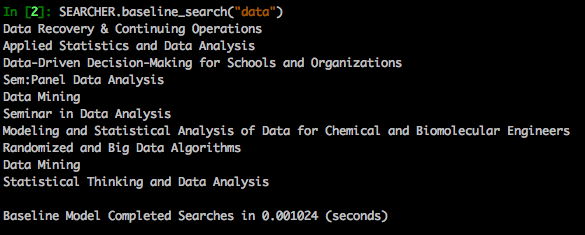
\includegraphics[width=\linewidth]{Images/1.png}
  \caption{Baseline Search.}
  \label{fig:baseline_search}
\end{figure}
Figure \ref{fig:baseline_search} shows rapid performance over query search.

In our SMART document vector modeled retrieval system, not only do we need to preprocess raw text documents as vectorized documents with term clustering/weighting to each course in the corpus, we need to transform a query as a vector with same dictionary used for courses corpus. After making a transformation, we would have to traverse each course in the corpus to calculate similarities using cosine similarity function and sort them by the scores. Hence the following are the bottleneck of computations for each query search.

\begin{enumerate}
\item Corpus to matrix transformation (TF-IDF, regional-term-weighting, term-clustering)
\item Query to vector transformation
\item Corpus to query similarity score calculation (for each N many courses in corpus)
\item Sorting corpus courses by similarity scores
\end{enumerate}

\begin{equation}
T = O(N * W) + O(M) + O( N * C (W, M) ) + O(N \log{N})
\end{equation}
Where $N$ is the number of courses in corpus and $W$ is the maximum number of words for a single course in corpus, $M$ is the token size of a query.

Obviously, this is a very expansive computation compared with simple query boolean search. Making it even worse, we need to constantly store/load a dicationary hash for vectorizing query which is $O(N * W)$. 

\begin{figure}
  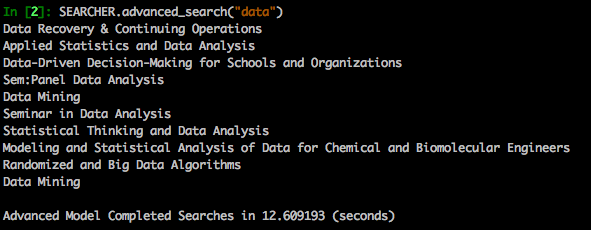
\includegraphics[width=\linewidth]{Images/2.png}
  \caption{Naive Advanced Search Implementation}
  \label{fig:naive_advanced_search}
\end{figure}
Figure \ref{fig:naive_advanced_search} shows very slow performance over naive course retrieval search implementation.

Naive implementation took ~$12.609$ seconds which is indeed $12607$ times slower. Even when took out the time to take preprocessing ~($10.753$ seconds), still took $1.856$ seconds which is $1856$ time slower than query boolean searching.

Therefore, we took the following optimization techniques to cut down retrieval complexity

\begin{enumerate}
\item Preprocess the corpus and store it to database
\item Serialize the dictionary hash and load only ONCE (loading takes ~1.5 seconds)
\item Use Map/Reduce function for any AND/OR operation such as boolean search or cosine similarity computation
\item Use Query Filtering to cut down course corpus to the courses that contains at least one query token in its vectorized course object.
\item Use Cache to store courses/queries terms that had been used before
\end{enumerate}

\begin{figure}
  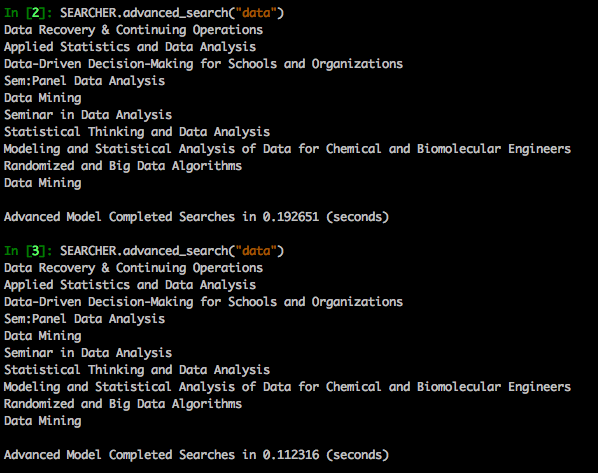
\includegraphics[width=\linewidth]{Images/3.png}
  \caption{Optimized Advance Search.}
  \label{fig:optimized_advance_search}
\end{figure}
Figure \ref{fig:optimized_advance_search} shows much better performance over advance search.

We were able to successfully optimize the query using the techniques above, and achieve much comprehensive query searching at the expense of only ~$10$ times slower computation than initial searching method. We observed that $0.112$ seconds is almost negligible to human-machine interaction user experience.

\vfill
\pagebreak

\section{Web Interface Integration and Usefulness}

Next task was to implement the retrieval model to search bar web interface on the current stack of Semester.ly. Successfully migrating the model implementation, you can see the difference from before to after implementation of new search system based on information retrieval techniques. With our advanced search, we were able to \textbf{process broader range} of queries upon courses database.

As you may be able to see from semester.ly's website, a web-interface looks as following:

\begin{figure}
  
\includegraphics[width=\linewidth]{Images/4.png}
  \caption{Semester.ly's Web Search Interface}
  \label{fig:semesterly search}
\end{figure}
Figure \ref{fig:optimized_advance_search} shows much better performance over advance search.

A search is made by passing a query through the search bar at top.

The following screenshots are some of the compare/contrast examples between baseline search and advanced search implementation.

\begin{figure}
    \centering
    \subfloat[baseline search 1]{{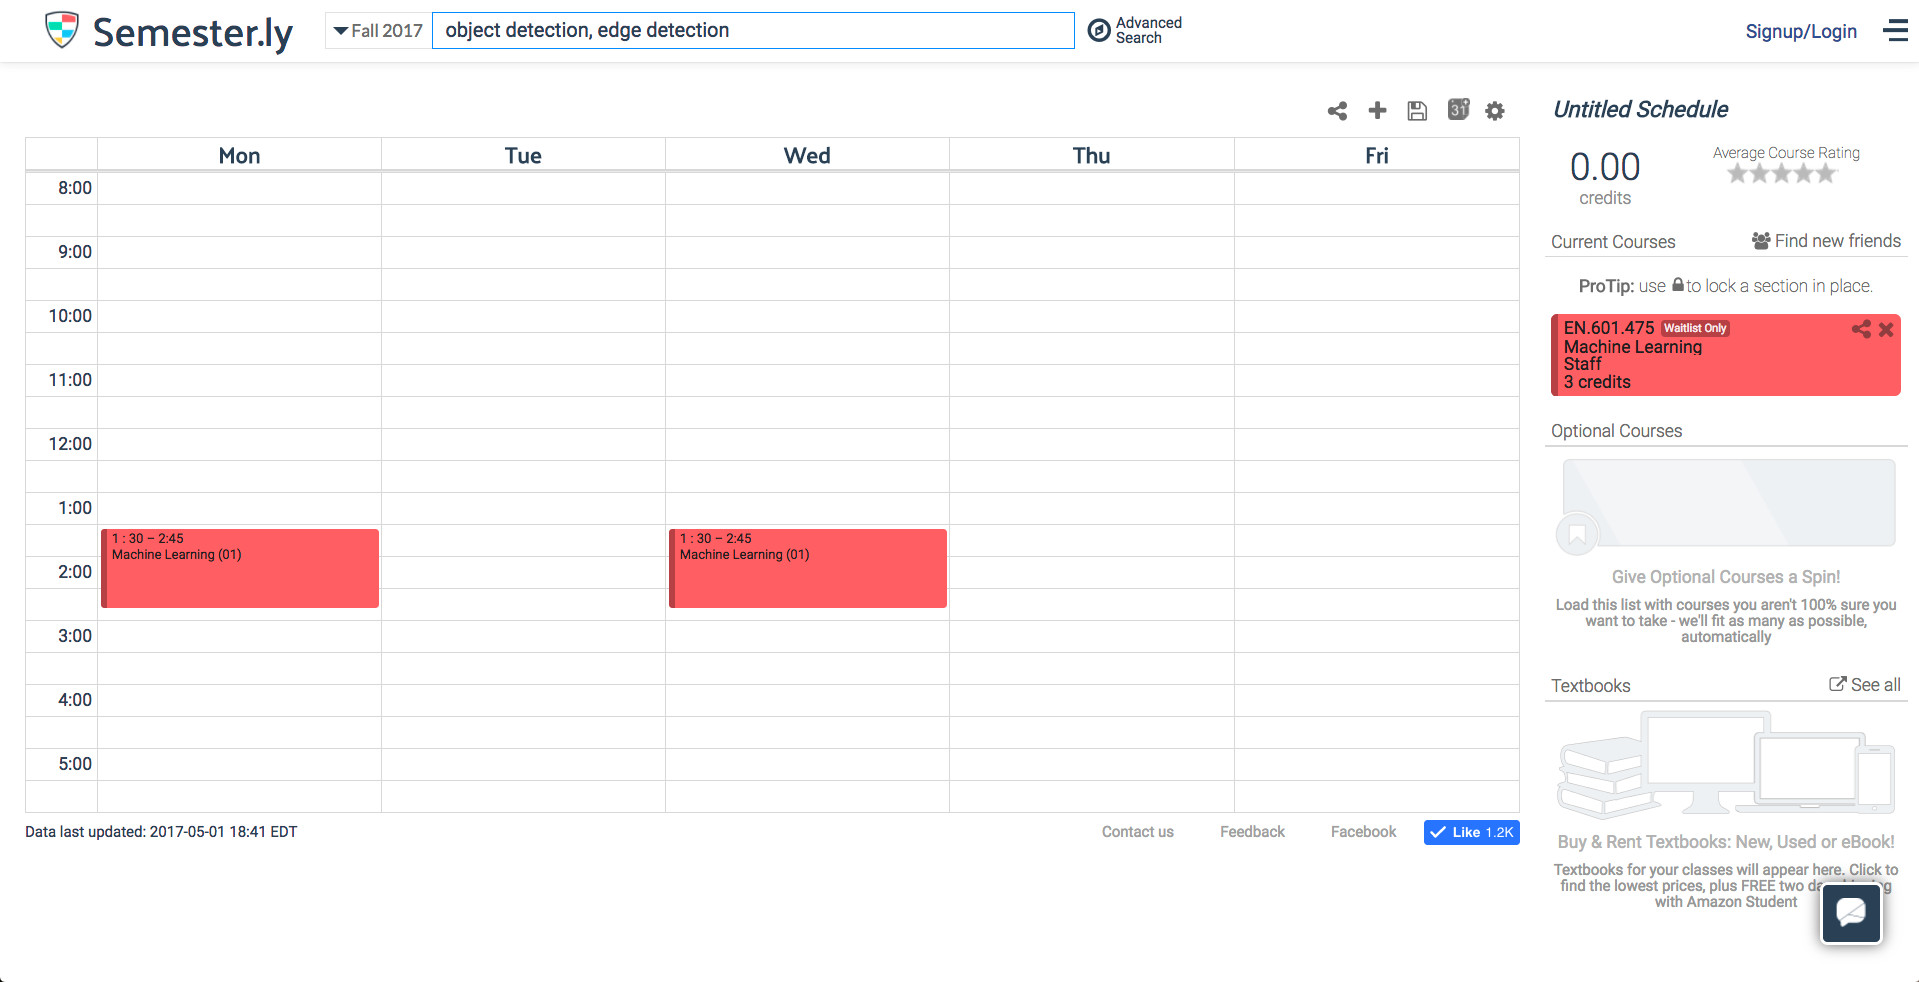
\includegraphics[width=7.5cm]{images/5_1.png} }}%
    \qquad
    \subfloat[advanced search 1]{{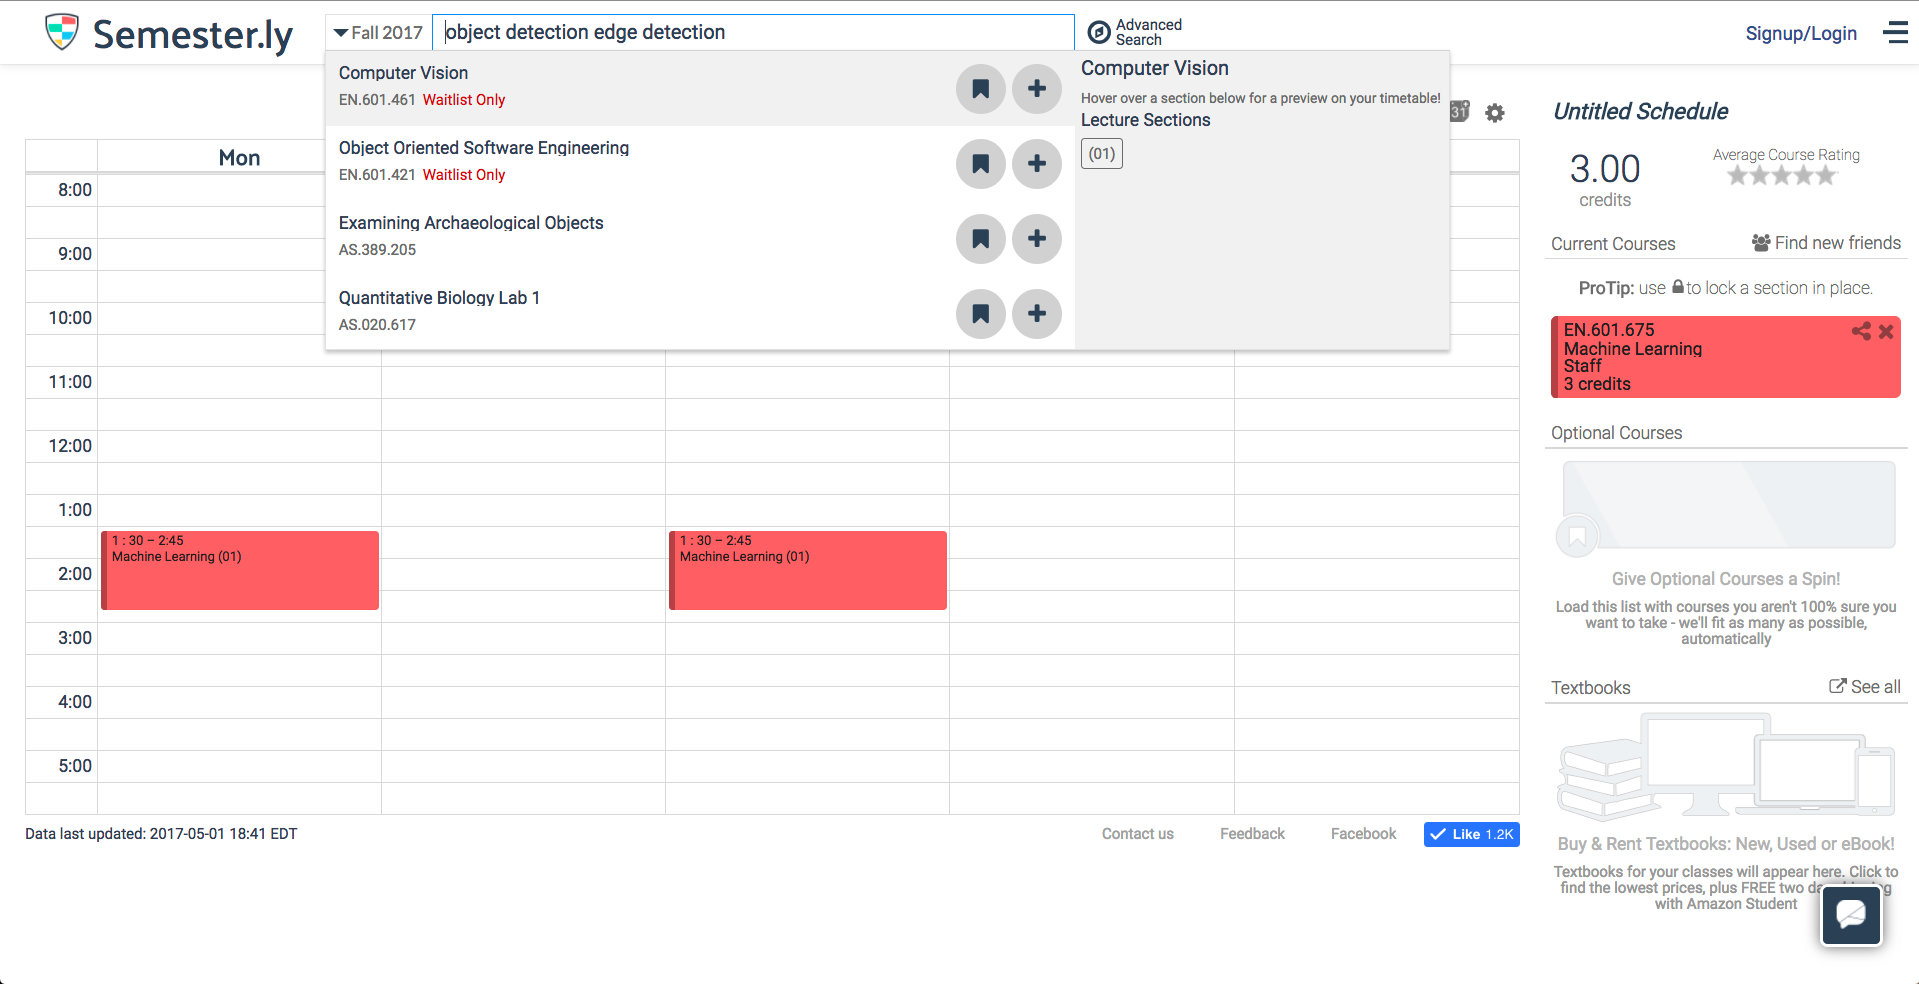
\includegraphics[width=7.5cm]{images/5_2.png} }}%
    \caption{Search results for \textbf{query 1:} object detection, edge detection} %
    \label{fig:comp1}%
\end{figure}

\begin{figure}
    \centering
    \subfloat[baseline search 2]{{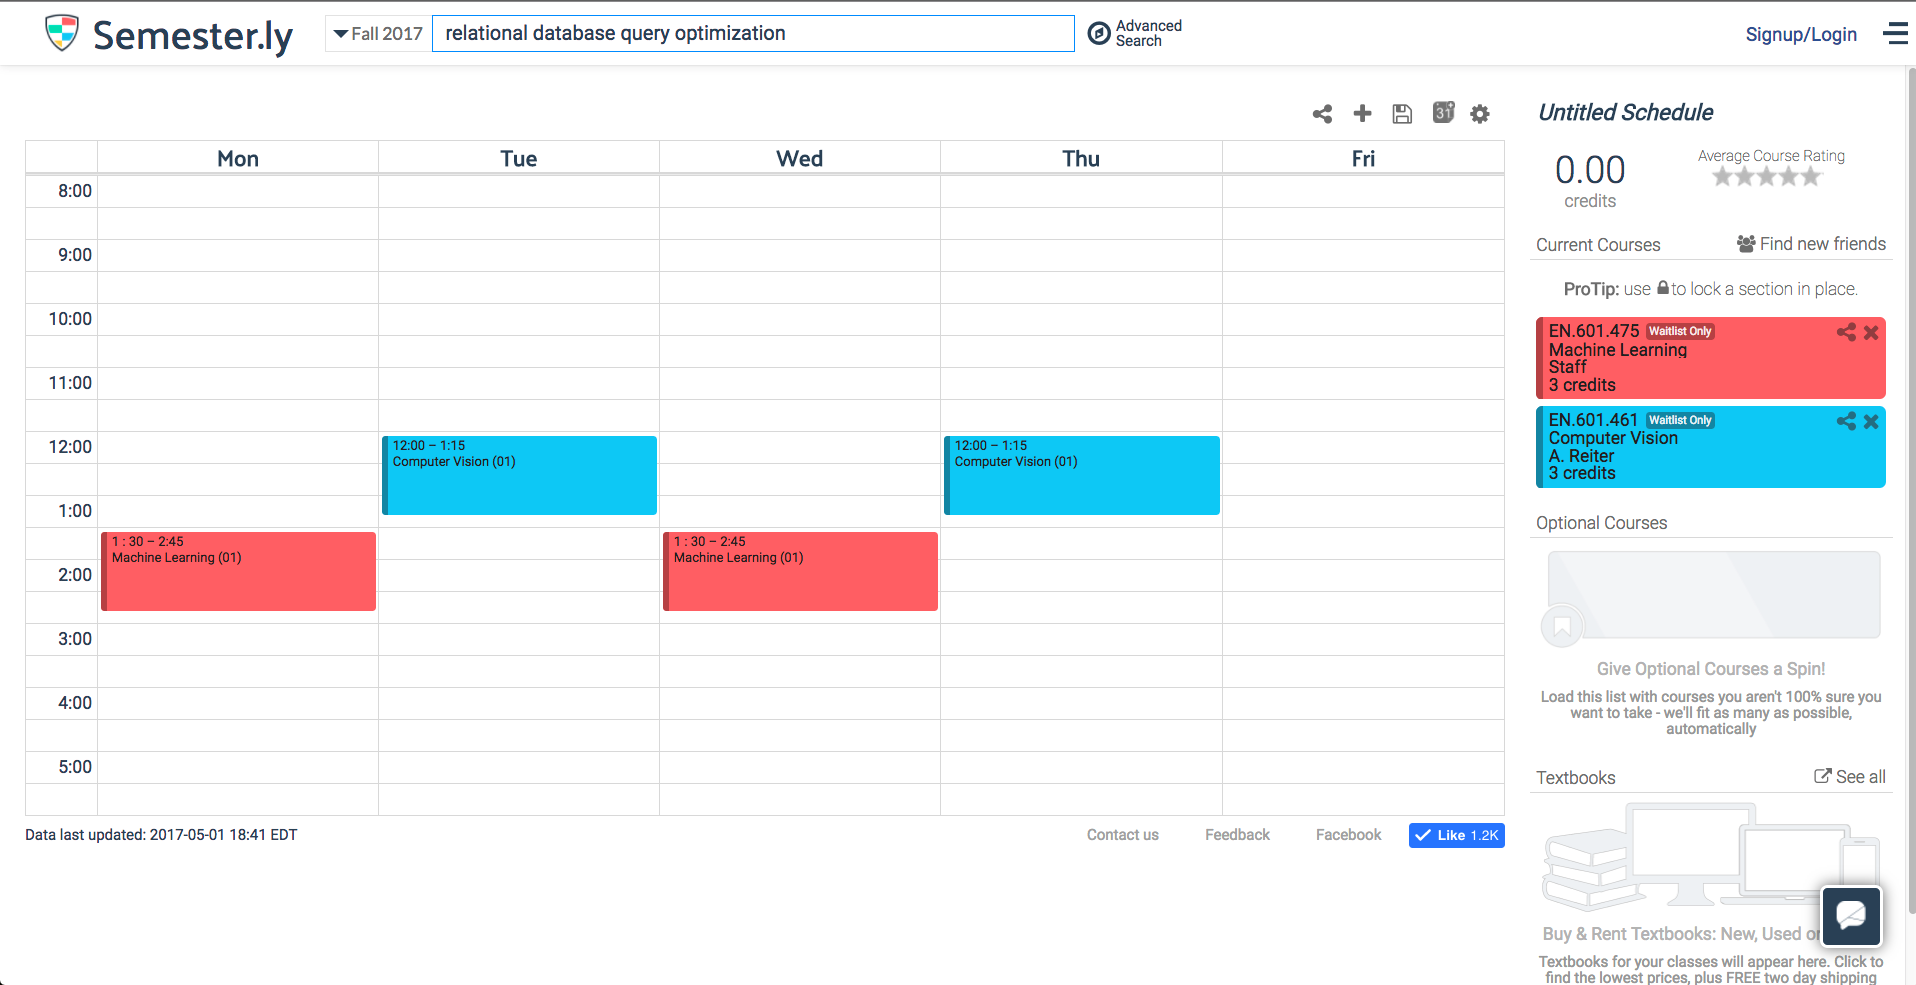
\includegraphics[width=7.5cm]{images/6_1.png} }}%
    \qquad
    \subfloat[advanced search 2]{{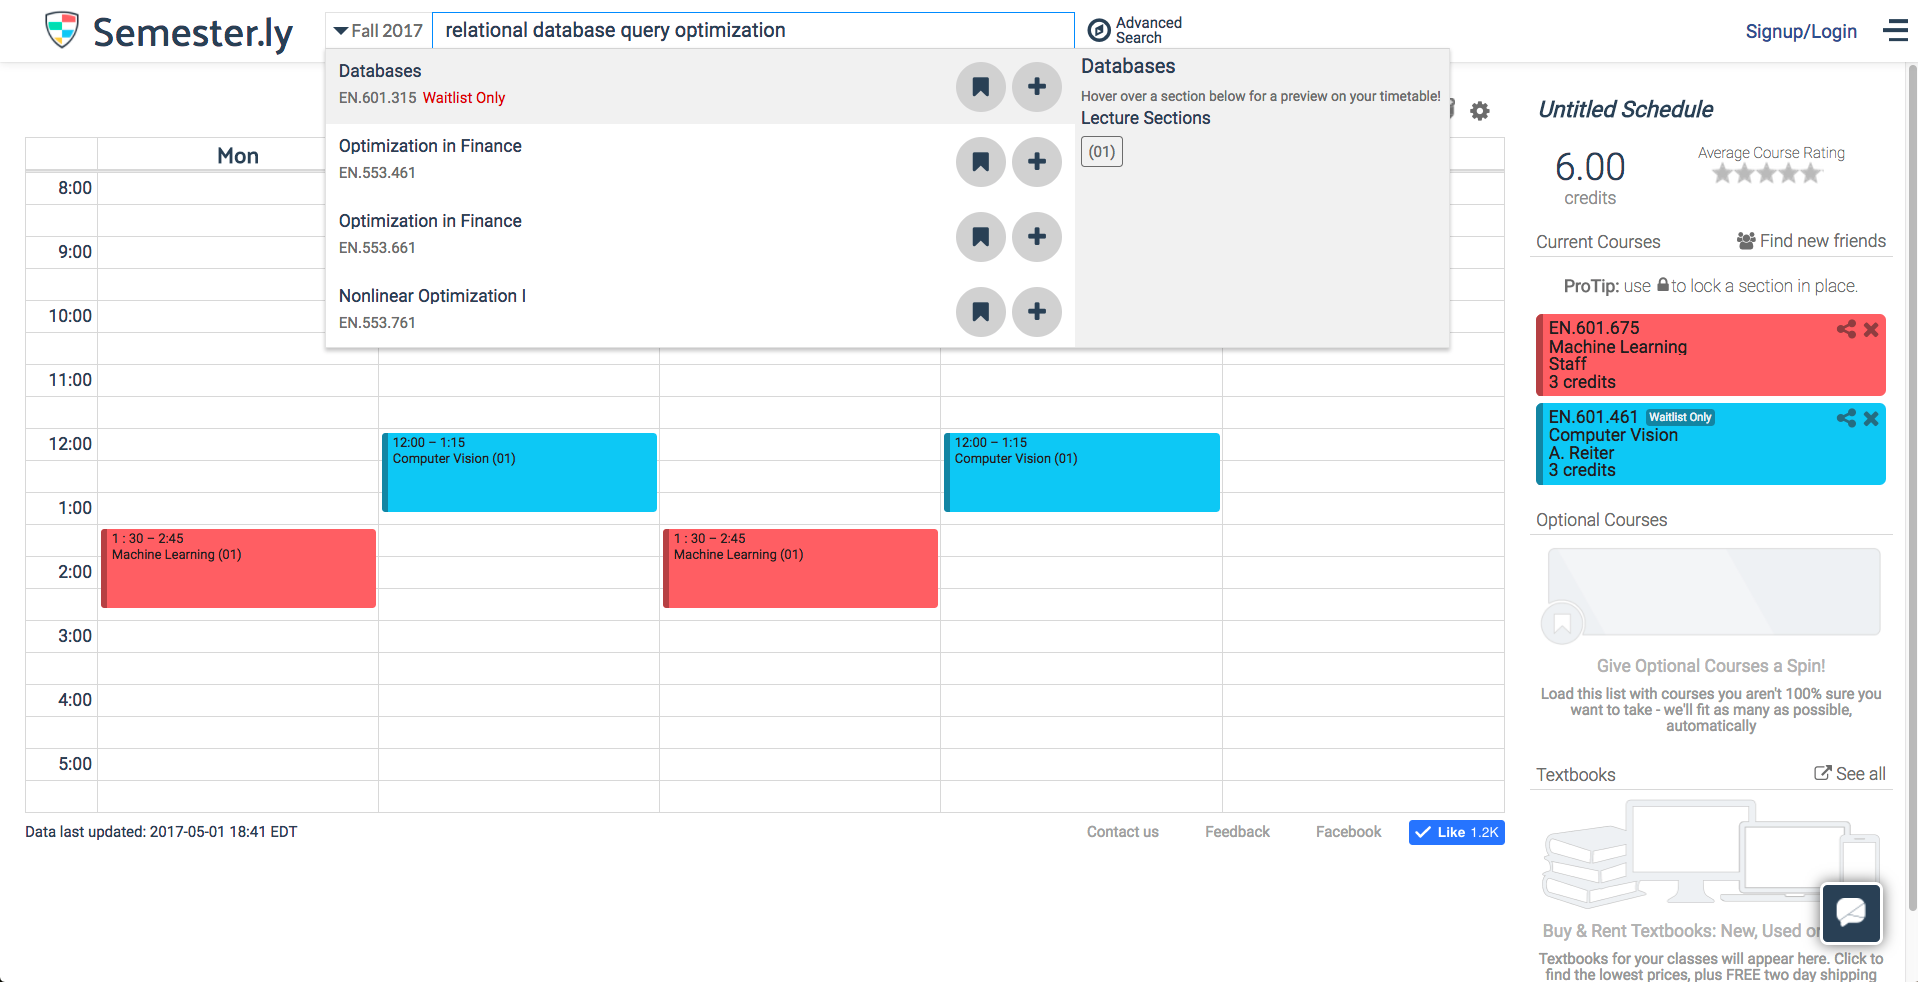
\includegraphics[width=7.5cm]{images/6_2.png} }}%
    \caption{Search results for \textbf{query 2:} relational database query optimization} %
    \label{fig:comp1}%
\end{figure}

\begin{figure}
    \centering
    \subfloat[baseline search 3]{{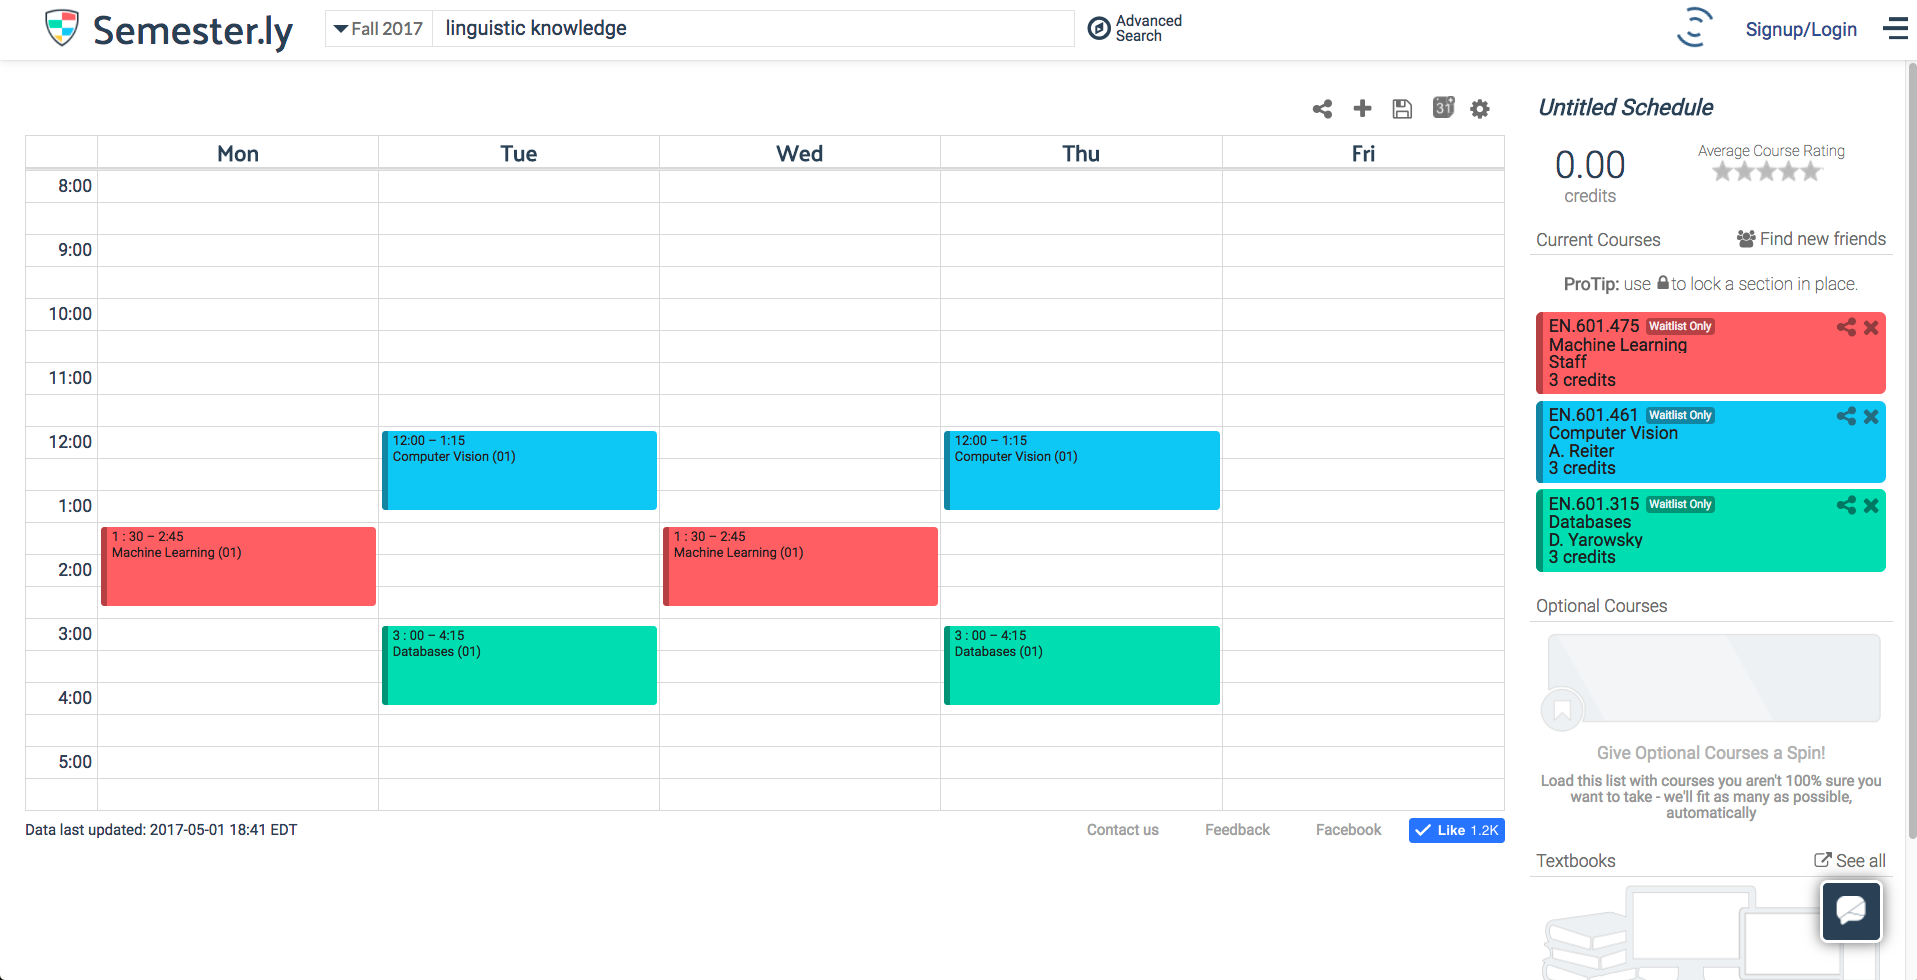
\includegraphics[width=7.5cm]{images/7_1.png} }}%
    \qquad
    \subfloat[advanced search 3]{{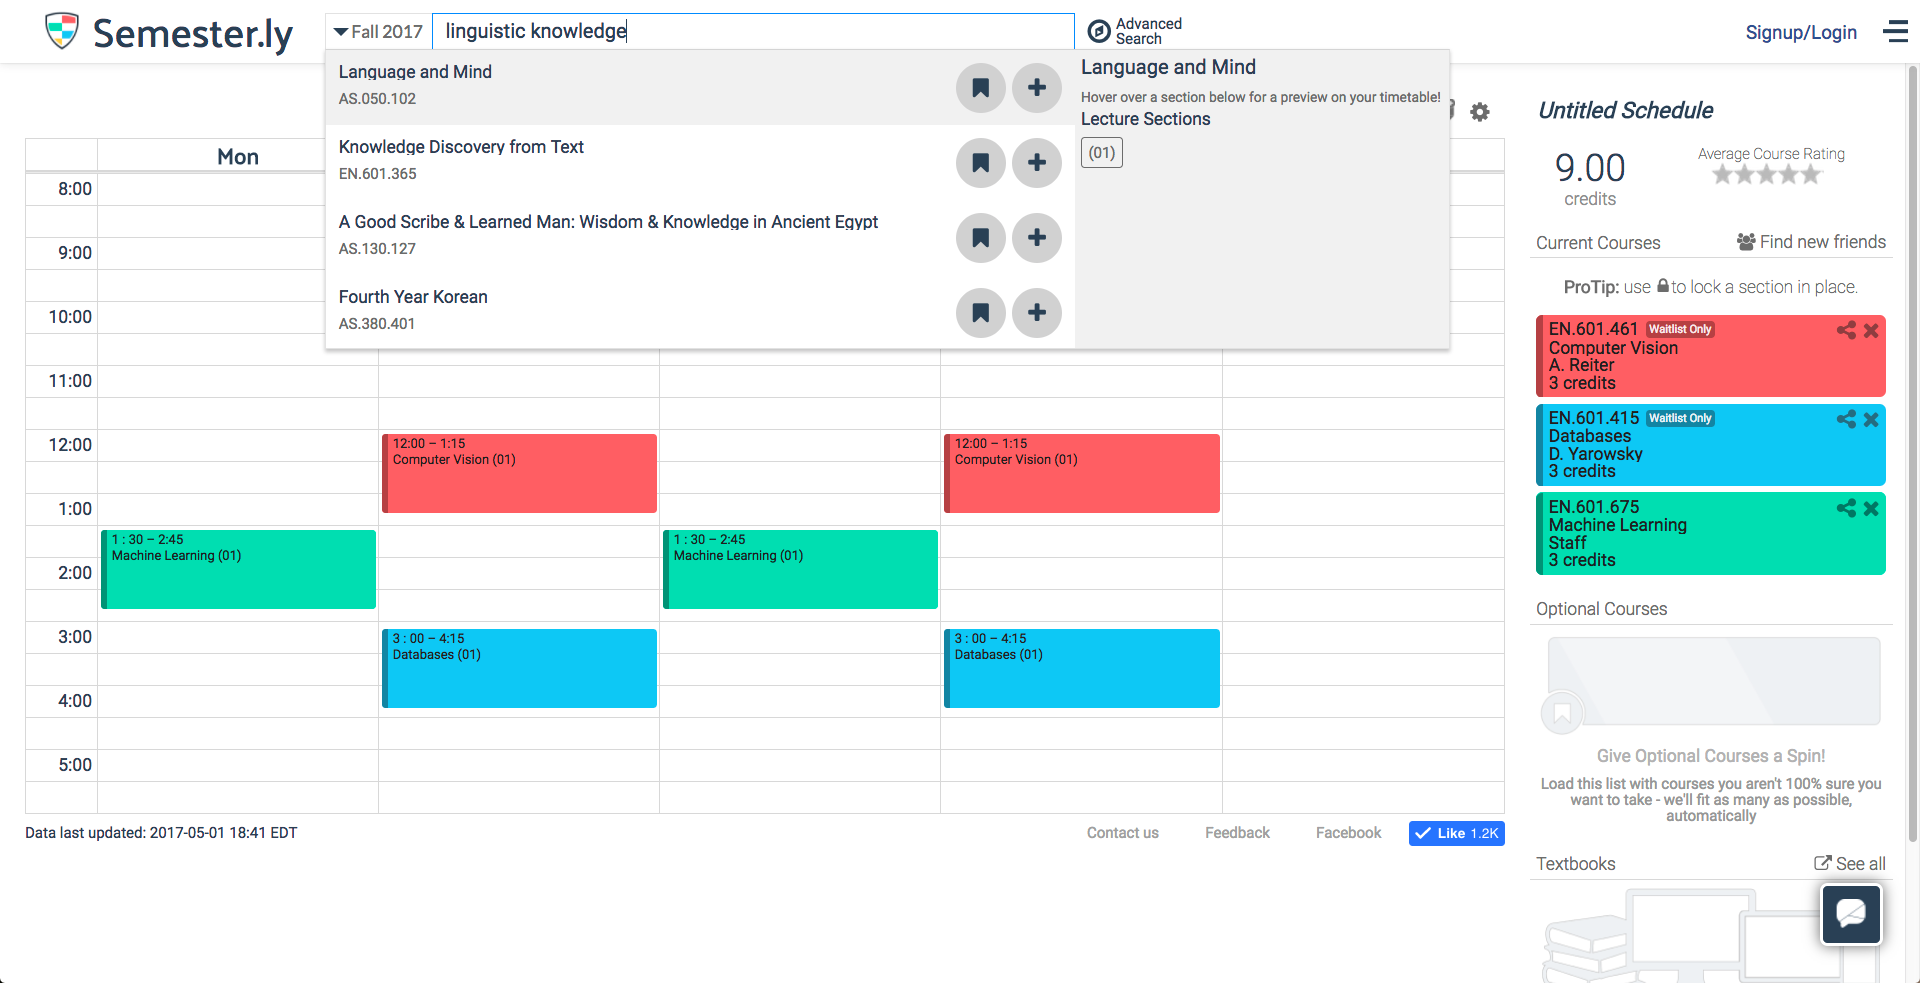
\includegraphics[width=7.5cm]{images/7_2.png} }}%
    \caption{Search results for \textbf{query 3:} linguistic knowledge} %
    \label{fig:comp1}%
\end{figure}

\pagebreak

Notice that most of the queries we tried indeed searches back no results in the baseline model. This is because no title matches all the tokens in a query we provided above, while advance search actually computes similarity scores between query and courses based on concurrent term occurances. One more advantage of the advanced search is that retrieved courses are \textbf{ordered by similarity/relevancy scores} which provides the \textbf{ranking}, while baseline search returns course objects in a storage order (i.e. alphabetical order), meaning there is no difference between retrieval orders.

Moving on, baseline search did not handle duplicate courses. In the advanced search, duplicate courses (duplicate names but with different codes) are handled in order to maximize usage of search result 'real estates', that are currently showing 4 retrieved courses. This allows users to retrieve diversified course results instead of a dominating match with multiple course levels (i.e. 3 'machine learning' courses with 400, 500, 600 level).

\begin{figure}
    \centering
    \subfloat[baseline search (not sorted)]{{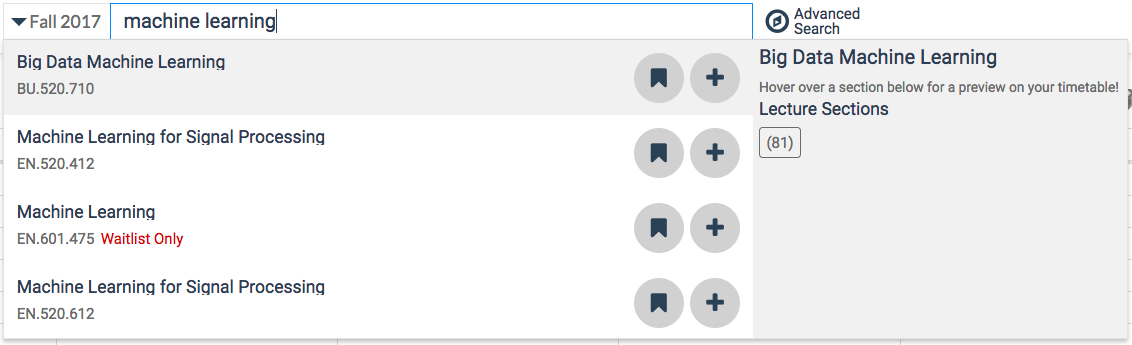
\includegraphics[width=7.5cm]{images/8_1.png} }}%
    \qquad
    \subfloat[advanced search (sorted by similarity scores)]{{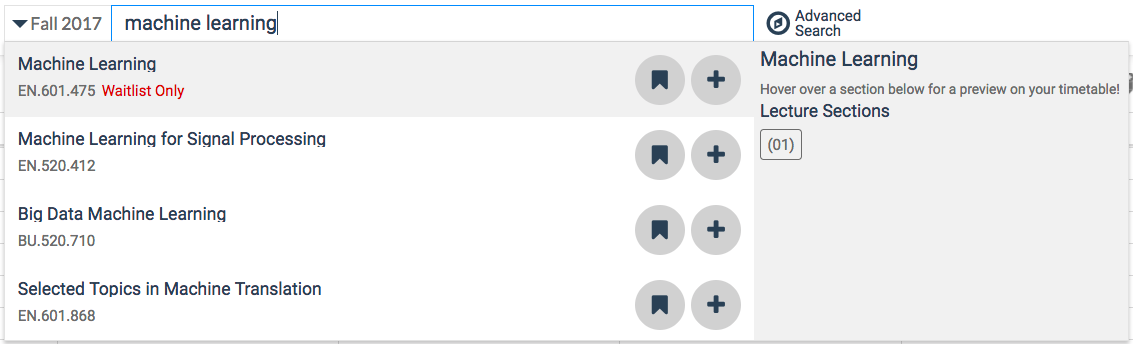
\includegraphics[width=7.5cm]{images/8_2.png} }}%
    \caption{Course retrieval ranking} %
    \label{fig:comp1}%
\end{figure}


\begin{figure}
    \centering
    \subfloat[baseline search (duplicacy not handled)]{{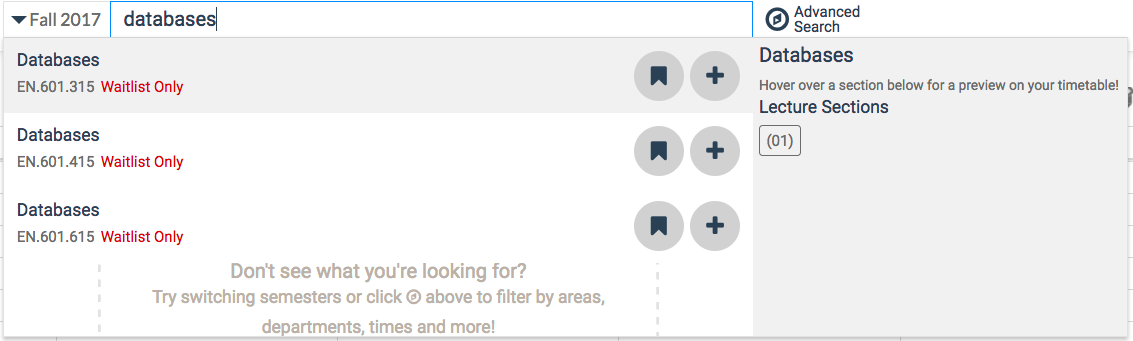
\includegraphics[width=7.5cm]{images/9_1.png} }}%
    \qquad
    \subfloat[advanced search (duplicacy handled)]{{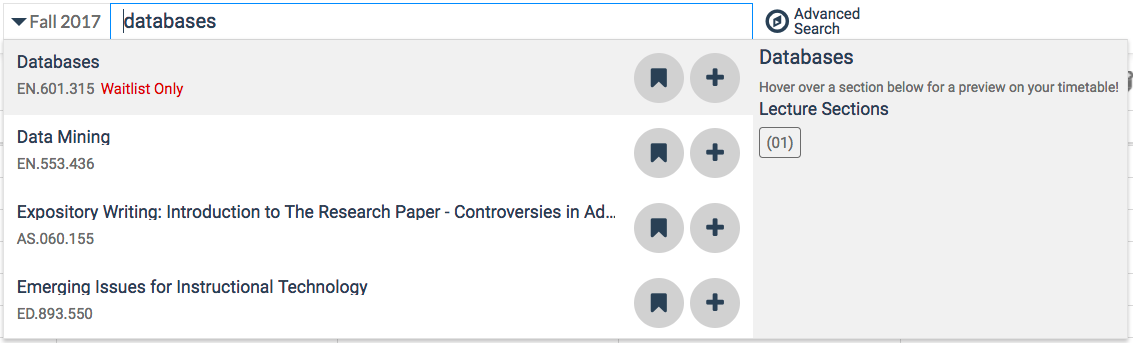
\includegraphics[width=7.5cm]{images/9_2.png} }}%
    \caption{Duplicate course handling} %
    \label{fig:comp1}%
\end{figure}

\vfill
\pagebreak

\section{Topic Modeling}

We wanted to further analyze the course distribution with respect to "topics". For example, a "Computer Ethics" class is a mix between "Computer Science" related topic and "Ethics" related topic. Through topic modeling of the courses corpus, we can transform each course vector as a vector distribution of topics, a kind of dimensionality reduction based on Latend Dirichilet Allocation (similar to PCA but more generative and probabilistic).

The following list of topics is the generated from LDA using $10$ number of topics, and $1000$ most used words.

\begin{verbatim}
Fitting LDA models with tf features, n_samples=2316 and n_features=1000...

Topics in LDA model:
Course Topic #0:
study independent theory independent study 110 algebra law topics linear introduction
Course Topic #1:
sec making engineering management decision risk financial business decision making product
Course Topic #2:
music digital performance sound art history open majors course students
Course Topic #3:
research students seminar faculty graduate required science project materials graduate students
Course Topic #4:
clinical course 110 care nr management practice students health advanced
Course Topic #5:
students course management learning issues learn teaching skills leadership development
Course Topic #6:
health public care health care public health environmental course nursing medical issues
Course Topic #7:
course students writing social reading class political language spanish contemporary
Course Topic #8:
course topics introduction include chemistry analysis materials theory methods topics include
Course Topic #9:
course design en students analysis systems data topics background computer
\end{verbatim}

As we can observe, notice that course topic $0$ reflects courses attributed for \textit{math theory independent study}, course topic $1$ reflects courses attributed with \textit{business management}, and course topic $6$ is most likely \textit{public health} classes.

Using these learned features, we provide functionalities such as \textbf{course clustering} and \textbf{retrieving similar courses}.

Indeed, in a closer look at these new representation of courses, a following transformations were made to the following courses with respect to $10$ topics distribution above:

\begin{enumerate}
\item \textbf{Quantitative Analysis of Clinical Data}\\
\begin{verbatim}
[ 0.00256473  0.00256479  0.00256418  0.00256417  0.00256429  0.00256424
  0.00256484  0.00256443  0.97691939  0.00256493]
\end{verbatim}
clearly, \textbf{topic $8$ (analysis methods)} is highly attributed.\\

\item \textbf{Vocal Coaching}\\
\begin{verbatim}
[ 0.03333333  0.03333333  0.69999977  0.03333333  0.03333333  0.03333357
  0.03333333  0.03333333  0.03333333  0.03333333]
\end{verbatim}
clearly, \textbf{topic $2$ (music)} is highly attributed.\\

\item \textbf{Investment-Portfolio Management}\\
\begin{verbatim}
[ 0.06707932  0.70831829  0.06027959  0.00625029  0.12681864  0.00625095
  0.00625032  0.00625133  0.00625042  0.00625085]
\end{verbatim}
clearly, \textbf{topic $1$ (business management)} is highly attributed.\\

\item \textbf{Honors Algebra I}\\
\begin{verbatim}
[ 0.95908301  0.00454574  0.00454641  0.00454745  0.00454594  0.00454659
  0.00454581  0.00454663  0.00454607  0.00454634]
\end{verbatim}
clearly, \textbf{topic $0$ (math theory independent study)} is highly attributed.\\
\end{enumerate}


The results even with $10$ number of topics, which is very small in number, show promising results and sign of potential.

\vfill
\pagebreak

\section{Course Clustering using LDA (topic feature transformation)}

After transforming each course object as a vector distribution of 50 different topics, we performed clustering method to analyze the general distribution of combinations of the topics under course corpus.

Specifically, we used \textbf{Gaussian Mixture Model} for clustering, with our assumption that courses with the same topic distribution would generally be spread out with gaussian-like (normal distribution) noise/error.

The following graph is the log likelihood plotting of the cluster distribution with respect to the number of $k$ clusters for GMM.

\begin{figure}
  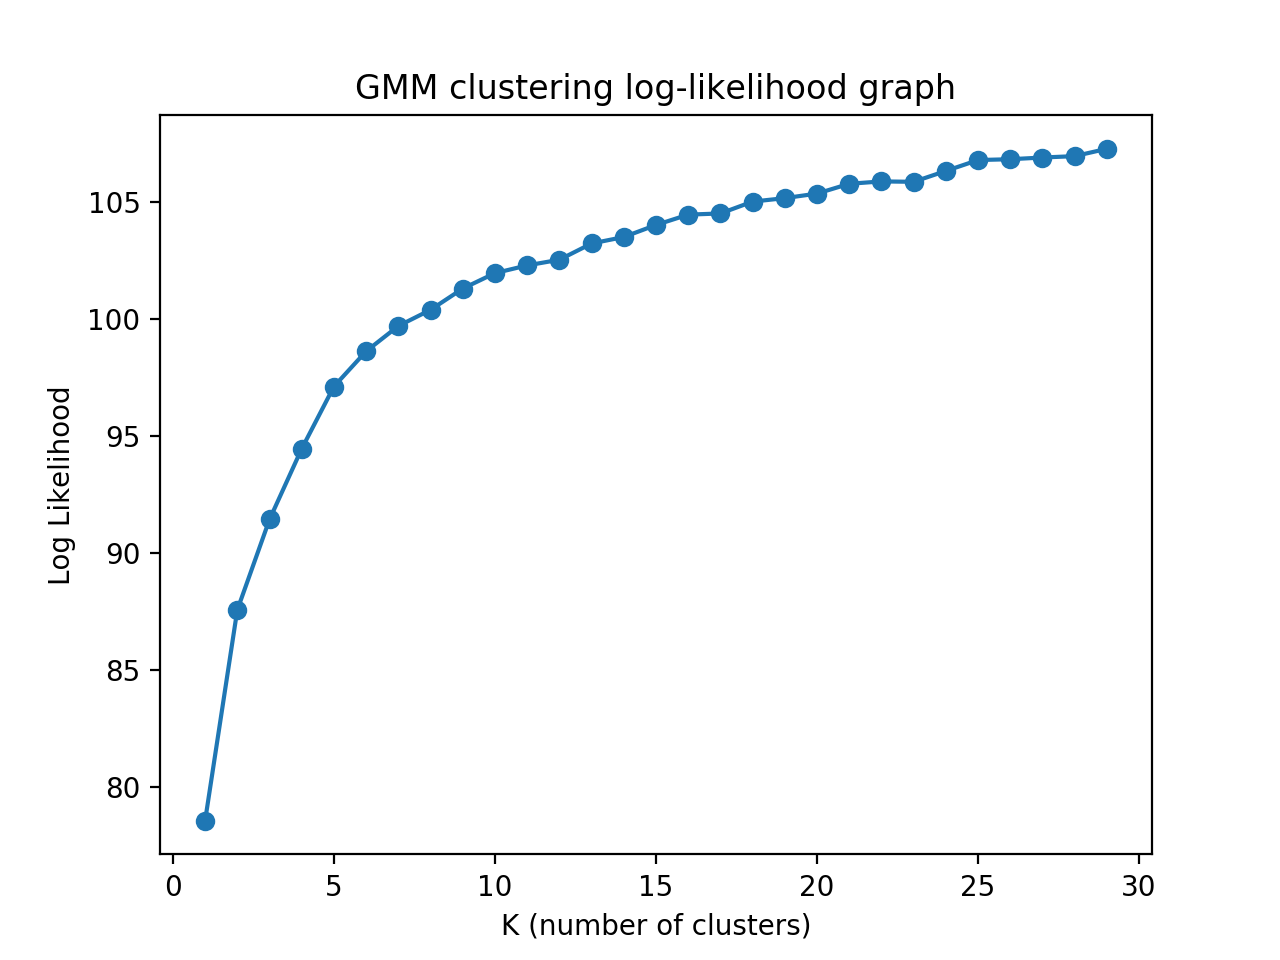
\includegraphics[width=\linewidth]{Images/10.png}
  \caption{GMM likelihood for each $k$ clusters}
  \label{fig:GMM_clustering}
\end{figure}
Figure \ref{fig:GMM clustering} shows general distribution/spread of courses in corpus.

As illustrated by the graph above, we observe that there are generally $10$ ~ $15$ different topic sets that are mostly spread out in courses corpus, which can be used especially for \textbf{complexity reduction}, truncating the search range, or providing \textbf{similar courses} under similar topics. Indeed, we may wish to further explore dimensionality reduction with the use of \textbf{Singular Value Decomposition} and \textbf{Principle Component Analysis} for feature transformation, then perform \textbf{Latend Semantics Analysis}. However, since topic modeling is rather much intuitive and easier to understand, we may expand the application of topic distribution for providing more information about each course, or for expansion of features such as classification, clustering and relevance calculation.


\section{Conclusion}
I believe that Semester.ly has created a positive impact on student bodies for facilitating a course scheduling process that can easily become overwhelming. I am an active user of Semester.ly myself and I remember being very impressed with all of its functionalities and constant dedications from developers. Through the project, I hoped to improve upon the user experience and user interface, in order to provide more flexible and comprehensive search engine for various applications and purposes.

I believe that the advanced search system will provide greater value to the current service, through providing a "virtual advisor" that can help students guide their curriculum at their schools. In the future, we wish to further expand its features including \textbf{user relevance feedback} on searches, \textbf{clustering} visualization of courses distribution, and providing most \textbf{similar courses}.

Furthremore, the system may enhance school's curriculum planning for each department through \textbf{user distribution prediction} for efficiency maximized course scheduling and planning, as well as providing more accurate descriptions for courses for better depicting each course.

I am incredibly grateful to the class \textit{Information Retrieval and Web Agent} for enabling me to explore various techniques under information extraction, and methods of applications for serving users. I wish to further expand on its system to add additional values, and integrate more technological tools for both college students and professors.

Lastly, I would like to thank professor David Yarowsky for his exceptionally knowledgeable lectures and support for carrying on throughout this project.

\end{document}





